\section{Additional experimental detail and ablations}
\label{app:ablations}

\subsection{Remaining setup detail}
\label{app:setup-full}
Under vLLM the returned sequences can diverge from the single-request runs, consistent with documented numerical and batching variability, and we treat those numbers as descriptive rather than as exact-equivalence evidence. Fitting time throughout excludes response generation, feature capture, model setup and export. One saved feature cache serves several fits, so its cost must not be charged to each fit separately.

\subsection{Where the trained parameters sit}
\label{app:placement}

\subsubsection{Where the trained parameters sit}
\label{sec:ablation-placement}
RelaySpec trains one map per feature stream and then folds those maps into the fusion block in front of which they sit. Because the folded result is a single matrix, the natural objection is that the factorization is irrelevant and any trainable matrix of the same size would do. Table~\ref{tab:ablation-placement} tests that, against four alternatives:

\begin{itemize}\itemsep1pt\parskip0pt
\item \textbf{Single fused projection.} One matrix of the same total size, trained in place of the five maps and initialized to exactly the function the five maps start from. This is the decisive control, since it differs from RelaySpec only in being unfactorized.
\item \textbf{Draft-transformer LoRA.} A rank-128 LoRA on the attention and MLP projections inside the draft blocks. This trains the drafter's body instead of its inputs, and is the established alternative that RelaySpec is meant to replace.
\item \textbf{Single joint map.} One dense matrix over all five concatenated streams, which permits mixing between streams at five times the parameters.
\item \textbf{Rank-$r$ maps.} Each whole map is replaced by a rank-$r$ product, rather than adding a low-rank correction to a retained full map.
\end{itemize}

\begin{table}[t]
\centering
\caption{Where the trained parameters sit, for fine-tuned Qwen3-4B targets under a matched accept-until-fail objective, 4{,}096 examples and 32 anchors. Values are percent gain in mean throughput over the unadapted drafter. HM is the harmonic mean of the corresponding speedup ratios and is the selection criterion. Best in each column in bold.}
\label{tab:ablation-placement}
\small
\begin{tabular}{lrrrrr}
\toprule
Trained object & Parameters & GSM8K & KiCad & NanoCoder & HM \\
\midrule
Five per-stream maps (RelaySpec) & 32.8M & $\mathbf{+37.6}$ & $+89.5$ & $+8.1$ & \textbf{1.376} \\
Single fused projection & 32.8M & $+32.4$ & $+44.5$ & $+8.2$ & 1.265 \\
Draft-transformer LoRA, rank 128 & 36.7M & $+36.4$ & $+75.5$ & $\mathbf{+9.8}$ & 1.355 \\
Single joint map over all streams & 163.8M & $+24.3$ & $\mathbf{+88.4}$ & $-7.0$ & 1.244 \\
Rank-128 maps & 3.3M & $+3.2$ & $+58.4$ & $-28.8$ & 0.999 \\
Rank-56 maps & 1.4M & $-21.9$ & $+35.1$ & $-49.3$ & 0.751 \\
Rank-28 maps & 0.7M & $-43.1$ & $+12.8$ & $-62.5$ & 0.565 \\
\bottomrule
\end{tabular}
\end{table}

\textbf{What this shows.} For scale, the unadapted drafter used as the 0\% reference here already reaches $3.3\times$ to $4.4\times$ autoregressive decoding before any adaptation (Table~\ref{tab:main}), so every percentage below is the further gain adaptation adds on top of that autoregressive speedup, not the whole story. The factorization does the work, not the parameter count. With identical parameters and an identical starting function, the single fused projection reaches a harmonic mean of 1.265 against 1.376 for the five maps and loses 45 points of gain on KiCad. The same contrast appears when transferring to Qwen3-8B, where under a matched objective the single fused projection reaches $0.365\times$ the native drafter on Math while the five maps reach $0.884\times$. Keeping one map per stream therefore changes what the optimizer can reach, even though the two parameterizations describe the same functions after folding and export as the same matrix. This is the behaviour that structural re-parameterization predicts, where a training-time factorization that merges away at inference still improves the trained result~\citep{huo2026repspec}. Replacing each whole map by a low-rank product degrades monotonically, and the two smallest ranks fall below the unadapted drafter, because replacing the map discards its ability to pass the original feature through rather than merely limiting the learned correction. Draft-transformer LoRA is competitive and wins on NanoCoder, so we do not claim that adapting inputs beats adapting the body on every workload. Its cost is that the draft transformer is no longer shared, which Section~\ref{sec:serving} shows is what makes the method useful in deployment.

\subsection{Whether the maps need to be nonlinear}
\label{app:capacity}

\subsubsection{Whether the maps need to be nonlinear}
\label{sec:ablation-capacity}
The maps are linear because a linear map changes the feature width and still folds into the fusion projection. To test whether that costs accuracy, we add a parallel nonlinear branch to each map, so stream $i$ contributes $W_ih_i+B_i\operatorname{SiLU}(A_ih_i)$~\citep{elfwing2018silu}, with $A_i$ reducing to 256 coordinates and $B_i$ initialized to zero. Training therefore starts at exactly the linear solution and departs from it only if that lowers the loss. The branch raises trained parameters from 32.8M to 39.3M for a fine-tuned target and from 52.4M to 60.9M for transfer, and unlike the linear map it cannot be folded away before inference. Table~\ref{tab:ablation-capacity} holds data, objective and schedule fixed within each setting.

\begin{table}[t]
\centering
\caption{Whether the maps need to be nonlinear. Values are mean tokens per second and acceptance length under matched data, objective and schedule. The nonlinear alternative carries 16 to 20 percent more parameters and remains an active computation at inference. Best in each row in bold.}
\label{tab:ablation-capacity}
\small
\begin{tabular}{llrrrrr}
\toprule
& & \multicolumn{2}{c}{Tokens/s} & & \multicolumn{2}{c}{$\tau$} \\
\cmidrule(lr){3-4}\cmidrule(lr){6-7}
Setting & Workload & Linear & Nonlinear & Change & Linear & Nonlinear \\
\midrule
Fine-tuned & GSM8K & \textbf{179.83} & 177.94 & $-1.05\%$ & \textbf{5.988} & 5.953 \\
 & KiCad & 312.47 & \textbf{321.76} & $+2.97\%$ & 11.256 & \textbf{11.411} \\
 & NanoCoder & \textbf{171.73} & 169.74 & $-1.16\%$ & \textbf{5.552} & 5.520 \\
\midrule
Replaced & Math & \textbf{220.26} & 215.71 & $-2.07\%$ & \textbf{7.984} & 7.980 \\
 & GSM8K & \textbf{176.87} & 174.56 & $-1.31\%$ & 6.242 & \textbf{6.257} \\
 & Code & 127.61 & \textbf{128.41} & $+0.63\%$ & 4.739 & \textbf{4.782} \\
 & Chat & \textbf{80.93} & 80.78 & $-0.20\%$ & 2.887 & \textbf{2.902} \\
\bottomrule
\end{tabular}
\end{table}

\textbf{What this shows.} The nonlinear branch is given every advantage, since it starts from the linear solution, carries more parameters and is selected by the optimizer only if it lowers the loss. It nevertheless changes throughput by between $-2.07\%$ and $+2.97\%$, leaves acceptance length almost unchanged, and is behind the linear map on five of the seven workloads. The linear form is therefore not a concession made for foldability. It is at least as accurate here and additionally collapses to one fixed matrix before inference. With differences of this size and one timed pass per cell we claim only that this nonlinear interface does not pay for itself.

\subsection{Two further objective controls}
\label{app:objective-extra}
First, on a separate matched architecture (a single low-rank fusion update rather than the five per-stream maps, held fixed to isolate the loss), plain uniform cross-entropy, the DFlash decaying weighting, and accept-until-fail were compared under identical data and schedule on NanoCoder: accept-until-fail reaches $1.072\times$ autoregressive decoding against $1.046\times$ for uniform cross-entropy and $1.047\times$ for decaying cross-entropy, a $2.4\%$ gain over uniform weighting that decaying weighting does not reproduce. This confirms that the prefix-aware accept-until-fail weighting, not merely having some position-dependent weighting, is what improves throughput. Second, for a fine-tuned target the training responses do not need to come from the fine-tuned target itself: fitting the same architecture from the base model's own generations reaches $1.001\times$ the throughput of fitting from the fine-tuned target's generations on the fine-tuned target's evaluation prompts, with a paired 95\% interval of $[0.995, 1.007]$ that contains 1. The gain therefore reflects adaptation to the workload distribution rather than a fit to the fine-tuned target's specific outputs.

\subsection{Serving many targets from one drafter}
\label{sec:serving}
Because the draft transformer is never trained, several adapted targets can share one copy of it, with only a small matrix differing between them. This is what draft-transformer LoRA gives up. Figure~\ref{fig:serving} measures the deployment on a vLLM server holding one target backbone and one draft backbone with three LoRA targets and frozen route assignments.

\begin{figure}[t]
    \centering
    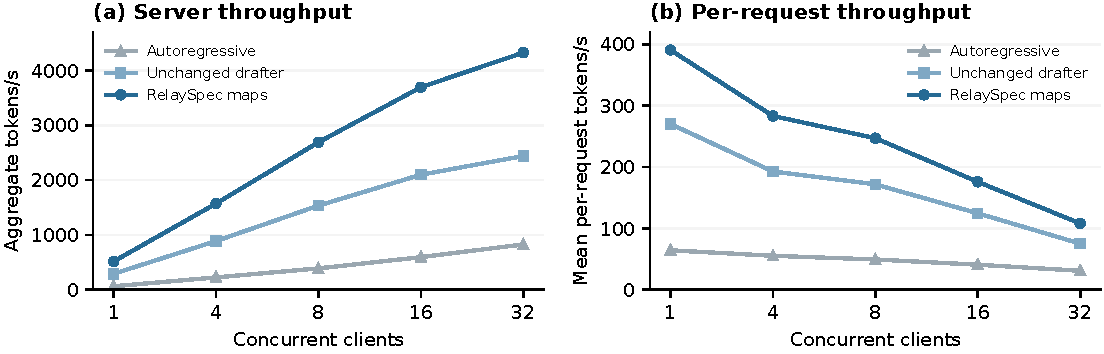
\includegraphics[width=\linewidth]{figures/relayspec_serving.pdf}
    \caption{One Qwen3-4B target backbone and one draft backbone serving three LoRA targets under vLLM on a single L40S, 384 requests with frozen route assignments. (a) aggregate throughput, total returned tokens divided by workload wall time including drain. (b) mean per-request throughput. The adapted drafter leads on server throughput at every concurrency, while per-request throughput falls with load for all three methods.}
    \label{fig:serving}
\end{figure}


\textbf{What this shows.} The single-request gains survive batching. Aggregate server throughput is higher for the adapted drafter at every concurrency measured, reaching 4{,}324 tokens per second against 2{,}440 for the unadapted drafter and 828 for autoregressive decoding at 32 clients, while acceptance length stays near 10.5 against 5.8. Panel (b) shows why both conventions must be reported: mean per-request throughput falls with load for all three methods even as server throughput rises, so a per-request number cannot stand in for a serving number. One pooled set of maps trained on the union of three domains reaches 98.9\% to 99.6\% of three separately trained sets across two repeats, so a deployment need not even hold one adapter per target. This is the practical form of the reuse question that motivates target-independent drafting~\citep{an2026pard2}. The advantage is not unbounded: on a Qwen3-8B server the adapted drafter leads at 1, 4 and 8 clients but falls within 4\% of the native drafter at 16 and 32 clients, because at high concurrency the bottleneck moves away from acceptance length.

\textbf{Concurrent serving across transfers.} The same question arises for a replaced target: does the transferred drafter still help once requests are batched under vLLM? Table~\ref{tab:transfer-serving} reports aggregate throughput at 16 concurrent clients for the three transfers with a published native drafter. Batching reproduces the single-request ordering of Table~\ref{tab:main} rather than changing it. On the transfer with the strongest single-request recovery, Qwen3-8B accelerated by the Qwen3-4B drafter, the mapped drafter leads on Math and GSM8K and trails narrowly on Code and Chat. On the reverse and cross-family transfers, where single-request recovery was already weaker, the mapped drafter trails the native drafter under concurrency on every workload, most on the cross-family Llama3.1-8B transfer. On the Llama3.2-3B transfer of Table~\ref{tab:llama-transfer}, the same server configuration reaches $2.53\times$, $3.08\times$, $1.71\times$ and $1.77\times$ autoregressive throughput on Math, GSM8K, Code and Chat at 16 clients.

\begin{table}[t]
\centering
\caption{Aggregate vLLM throughput at 16 concurrent clients, total returned tokens divided by workload wall time including drain. Bold marks the higher of native and mapped.}
\label{tab:transfer-serving}
\small
\begin{tabular}{llrrr}
\toprule
Target $\leftarrow$ drafter & Workload & Native (tok/s) & Mapped (tok/s) & Mapped/native \\
\midrule
Qwen3-8B $\leftarrow$ Qwen3-4B & Math & 2524.31 & \textbf{2716.26} & 1.076 \\
 & GSM8K & 2207.43 & \textbf{2262.03} & 1.025 \\
 & Code & \textbf{1748.19} & 1548.47 & 0.886 \\
 & Chat & \textbf{1091.14} & 1065.93 & 0.977 \\
\midrule
Qwen3-4B $\leftarrow$ Qwen3-8B & Math & \textbf{4482.42} & 3710.76 & 0.828 \\
 & GSM8K & \textbf{3160.99} & 3078.87 & 0.974 \\
 & Code & \textbf{2840.15} & 2002.79 & 0.705 \\
 & Chat & \textbf{1888.69} & 1431.21 & 0.758 \\
\midrule
Llama3.1-8B $\leftarrow$ Qwen3-4B & Math & \textbf{1894.99} & 1046.94 & 0.553 \\
 & GSM8K & \textbf{1354.50} & 853.13 & 0.630 \\
 & Code & \textbf{1296.83} & 636.97 & 0.491 \\
 & Chat & \textbf{1440.04} & 524.40 & 0.364 \\
\bottomrule
\end{tabular}
\end{table}

\textbf{Memory and GPU usage.} We measured post-request allocated and reserved GPU memory on the same T1 serving cells above. Allocated memory rises from 30.5914 GiB for the native drafter to 30.9190 GiB for the mapped drafter, a constant 0.33 GiB increase regardless of workload or concurrency; reserved memory shows the same small, workload-independent gap. This matches expectation: the trained maps add 52.4 million BF16 parameters to an 8-billion-parameter target and a several-billion-parameter draft transformer, so the memory cost of adaptation is negligible relative to the models it accelerates, and it does not grow with client count.

\subsection{EAGLE-3 generalization}
\label{app:eagle-table}
\begin{table}[t]
\centering
\caption{Generalization to EAGLE-3, using three input maps. Token supervision is used for a fine-tuned target and reconstruction for a replaced one, following the selection in Section~\ref{sec:ablation-objective}. The reference is the unadapted EAGLE-3 drafter for the fine-tuned block and a published EAGLE-3 drafter native to Qwen3-8B for the replaced block. Best in each row in bold. Acceptance uses EAGLE-3's upstream counters and is not comparable with the DFlash tables.}
\label{tab:eagle}
\small
\begin{tabular}{llrrrrr}
\toprule
& & \multicolumn{2}{c}{Tokens/s} & & \multicolumn{2}{c}{$\tau$} \\
\cmidrule(lr){3-4}\cmidrule(lr){6-7}
Setting & Workload & Reference & RelaySpec & $\times$ref & Reference & RelaySpec \\
\midrule
Fine-tuned Qwen3-4B, & GSM8K & 71.19 & \textbf{120.35} & \textbf{1.69} & 3.347 & \textbf{5.695} \\
token supervision & NanoCoder & 81.77 & \textbf{119.30} & \textbf{1.46} & 3.852 & \textbf{5.668} \\
 & KiCad & 73.82 & \textbf{151.86} & \textbf{2.06} & 3.794 & \textbf{7.363} \\
\midrule
Qwen3-8B from Qwen3-4B, & Math & 72.18 & \textbf{77.99} & \textbf{1.08} & 3.627 & \textbf{3.638} \\
reconstruction & GSM8K & 75.58 & \textbf{80.59} & \textbf{1.07} & 3.713 & \textbf{3.840} \\
 & Code & 63.88 & \textbf{65.53} & \textbf{1.03} & \textbf{3.351} & 3.293 \\
 & Chat & 61.82 & \textbf{63.41} & \textbf{1.03} & \textbf{3.186} & 3.136 \\
\bottomrule
\end{tabular}
\end{table}

\subsection{Training examples required}
\label{app:cost-table}
\begin{table}[t]
\centering
\caption{Training examples required, against the published DFlash recipe of about 800{,}000 samples~\citep{chen2026dflash}. Every fit here runs on two L40S GPUs in under half an hour.}
\label{tab:cost}
\small
\begin{tabular}{lrr}
\toprule
Setting & Training examples & Reduction vs. published DFlash \\
\midrule
Fine-tuned target (DFlash, five maps) & 4{,}096 & 195$\times$ fewer \\
Replaced target (DFlash, five maps) & 16{,}384 & 49$\times$ fewer \\
Fine-tuned target (EAGLE-3, three maps) & 4{,}096 & 195$\times$ fewer \\
Replaced target (EAGLE-3, three maps) & 16{,}384 & 49$\times$ fewer \\
\bottomrule
\end{tabular}
\end{table}

\subsection{Greedy verification}
\label{app:greedy}
\textbf{Greedy verification.} For greedy decoding, changing the drafter does not change the target's output if block verification makes the same choices as sequential target evaluation on identical prefixes. To see this, assume that the committed prefix matches autoregressive decoding. Each accepted proposal equals the target's next choice, and the first rejected proposal is replaced by that choice. If all proposals are accepted, the target supplies the next token. The extended prefix therefore still matches, and induction establishes the result for the complete sequence~\citep{leviathan2023speculative,chen2023sampling}. This argument assumes consistent token handling, stopping rules, and target evaluation.

\subsection{Llama3.2-3B transfer}
\label{app:llama-table}
\begin{table}[t]
\centering
\caption{Llama3.1-8B drafter reused for Llama3.2-3B. Speedup is relative to autoregressive decoding (AR), the same $1.00\times$ baseline convention as Table~\ref{tab:main}.}
\label{tab:llama-transfer}
\small
\begin{tabular}{lrrr}
\toprule
Workload & AR (tok/s) & Speedup & $\tau$ \\
\midrule
Math & 61.90 & 2.35$\times$ & 4.78 \\
GSM8K & 64.45 & 2.18$\times$ & 4.16 \\
Code & 63.09 & 1.88$\times$ & 3.44 \\
Chat & 64.73 & 1.61$\times$ & 2.97 \\
\bottomrule
\end{tabular}
\end{table}

\subsection{Public-runtime comparison}
\label{app:public-runtime}
\begin{table}[t]
\centering
\caption{Public-runtime comparison on 128 MATH development questions, 2{,}048-token cap. Speedup is each system's own end-to-end throughput divided by its own autoregressive throughput, with a paired 95\% bootstrap interval. This uses the earlier single-projection interface, not the five-map DFlash construction evaluated elsewhere in this section, and different runtimes and inherited base models prevent attributing the ranking to the adaptation method alone. Bold marks the highest observed speedup.}
\label{tab:public-runtime}
\small
\begin{tabular}{lrrr}
\toprule
System & End-to-end (tok/s) & Own AR (tok/s) & Speedup [95\% CI] \\
\midrule
Single-projection interface & 193.68 & 37.72 & \textbf{5.14 [4.90, 5.37]} \\
PARD & 105.63 & 31.67 & 3.34 [3.22, 3.45] \\
SD$^2$ (frozen drafter) & 19.92 & 12.48 & 1.60 [1.56, 1.63] \\
\bottomrule
\end{tabular}
\end{table}

\subsection{Objective ablation}
\label{app:objective-table}
\label{sec:ablation-objective}
\begin{table}[t]
\centering
\caption{Which objective trains the maps. The upper block reports throughput relative to the unadapted drafter for fine-tuned Qwen3-4B targets. The lower block reports throughput relative to the native Qwen3-8B drafter for transfer from Qwen3-4B, on the matched 8{,}192-example fits. MSE50 and MSE100 supervise that fraction of prompt and response positions. Best in each column in bold. HM is the selection criterion.}
\label{tab:ablation-objective}
\small
\begin{tabular}{llrrrrr}
\toprule
Setting & Objective & \multicolumn{4}{c}{Workload} & HM \\
\midrule
 & & GSM8K & KiCad & NanoCoder & & \\
\cmidrule(lr){3-5}
Fine-tuned & Accept-until-fail & \textbf{1.376} & 1.895 & \textbf{1.081} & & \textbf{1.376} \\
 & Decaying cross-entropy & 1.368 & \textbf{1.935} & 1.031 & & 1.353 \\
 & Reconstruction, MSE50 & 1.011 & 1.191 & 0.977 & & 1.052 \\
\midrule
 & & Math & GSM8K & Code & Chat & \\
\cmidrule(lr){3-6}
Replaced & Reconstruction, MSE100 & 0.998 & \textbf{0.990} & 0.828 & \textbf{0.891} & \textbf{0.921} \\
 & Reconstruction, MSE50 & \textbf{0.999} & 0.975 & \textbf{0.832} & 0.888 & 0.919 \\
 & Decaying cross-entropy & 0.886 & 0.919 & 0.406 & 0.573 & 0.623 \\
 & Accept-until-fail & 0.884 & 0.911 & 0.385 & 0.558 & 0.604 \\
\bottomrule
\end{tabular}
\end{table}

\subsection{Supervision budget}
\begin{figure}[t]
    \centering
    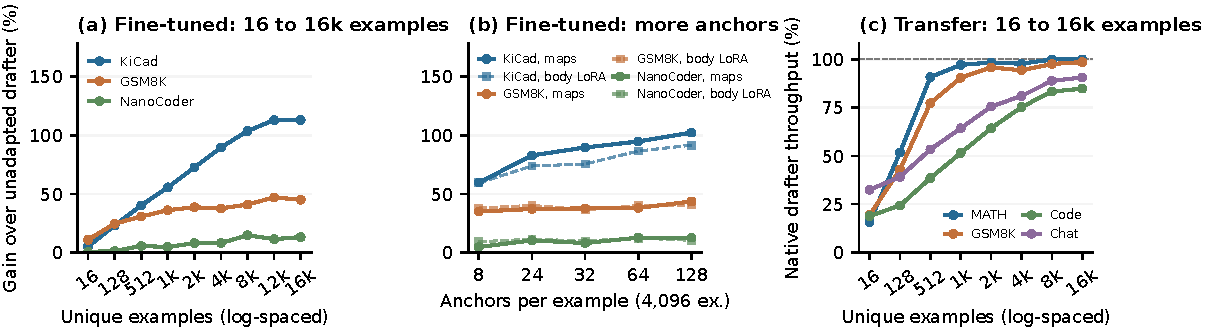
\includegraphics[width=\linewidth]{figures/relayspec_scaling.pdf}
    \caption{Supervision budget in both settings, from 16 to 16{,}384 training examples. (a) and (c) share a log-spaced example axis; (b) fixes examples at 4{,}096 and varies anchors per example. (a) and (b) use fine-tuned Qwen3-4B targets with the accept-until-fail objective, where solid lines train the five interface maps and dashed lines train a rank-128 LoRA inside the draft transformer. (c) transfers the Qwen3-4B drafter to Qwen3-8B with the reconstruction objective and plots throughput as a percentage of the native Qwen3-8B drafter. Adaptation is already effective at 16 examples and speedup keeps improving with supervision without saturating at the largest budget measured.}
    \label{fig:scaling}
\end{figure}


\subsection{EAGLE-3 recurrent objective}
\label{app:eagle-method}
\subsection{Extension to EAGLE-3}
\label{sec:method-eagle}
The construction is not specific to DFlash. EAGLE-3 combines features from three target layers before autoregressive drafting~\citep{li2025eagle3}, so $K=3$. We place one map before each of those inputs and leave the original feature projection, prediction network, and autoregressive drafting procedure unchanged. The maps fold into that projection exactly as in Equation~\ref{eq:folded-fusion}, so inference again runs the original architecture with one updated projection.

We pair each setting with the same objective we use for DFlash. For a LoRA-adapted target the feature widths match, so the maps start at the identity and receive token supervision. Because EAGLE-3 drafts one token at a time instead of filling a masked block, we apply the accept-until-fail rule along its own recurrent path. At each sampled anchor the drafter predicts up to eight successive tokens, a position is supervised only when every earlier prediction was correct, and the first incorrect prediction is still supervised. A saved token continues a path only where it matches the greedy prediction. The frozen drafter carries a reduced vocabulary head, so a target token outside that head ends a path without contributing a loss term, and we normalize each example by its own count of supervised positions. For a replaced target the widths can differ, so the maps start at Xavier-uniform values and train by reconstruction using Equation~\ref{eq:mse-method}.


